%\section{Evaluation}\label{sec:evaluation}
%
%In this section, a quantitative evaluation of the proposed streaming tree cut algorithm is conducted.
%%The usefulness of our approach is then demonstrated with two case studies.
%The usefulness of \kg{the} approach is then demonstrated with two case studies.

%\subsection{Quantitative Evaluation}
\section{Quantitative Evaluation}
\label{sec:quantitativeevaluation}
%To assess the effectiveness of our streaming tree cut algorithm, we performed experiments on a number of different datasets.
In this section, a quantitative evaluation of the proposed streaming tree cut algorithm is conducted.

%\subsubsection{Criteria}

\subsection{Fitness and Smoothness}
%To assess the effectiveness of \kg{the} streaming tree cut algorithm, \kg{we conducted} experiments on \kg{several} datasets.
To assess the effectiveness of \kg{the} streaming tree cut algorithm, we \tvcgminor{compared our algorithm with a baseline algorithm in terms of fitness and smoothness.}

\subsubsection{Criteria}
%Fitness and smoothness were employed as two important criteria to evaluate the derived streaming tree cuts.
%The fitness measures how satisfactorily the topics on the tree cut represent the topic distribution within a topic tree.
Fitness and smoothness \kg{are} two important criteria to evaluate the derived streaming tree cuts.
\dc{Fitness} measures how satisfactorily the topics on the tree cut represent the topic distribution within a topic tree.
%The fitness measures \kg{the satisfactory representation of} the topic distribution within \kg{the topics on the tree cut}.

\noindent\textbf{\normalsize Fitness ($\bm{F}$)}:
We derived the measure from the proposed tree cut likelihood equation, $\bm{F}=p({\phi}^t|T^t)p(\mathcal{D}_{f}|{\phi}^t)$,
%\kg{The} metric from the proposed tree cut likelihood equation, $\bm{F}=p({\phi}^t|T^t)p(D_{f}|{\phi}^t)$, \kg{is derived,}
where the right side is defined in Eq.~(\ref{eq:hmm2}).
%$p({\phi}^t|T^t)$ describes how the tree cut fits the focus and $p(\mathcal{D}_{f}|{\phi}^t)$ describes how it fits the tree.
$p({\phi}^t|T^t)$ describes how the tree cut \xiting{fits} the tree and $p(\mathcal{D}_{f}|{\phi}^t)$ describes how it \xiting{fits} the focus.
%$p({\phi}^t|T^t)$ describes \kg{the fit of} the tree cut \kg{and} the focus. $p(D_{f}|{\phi}^t)$ describes \kg{the} fit \kg{of} the tree.
%The larger the $F$ value, the better the tree cut.
A larger  $F$ value \kg{indicates a} better tree cut.

%Accordingly, likelihood was utilized to measure the fitness of a tree.
%The following three metrics were introduced to assess the smoothness between adjacent tree cuts.
The following three measures \kg{assess} the smoothness between \kg{the} adjacent tree cuts.
%In our implementation, the larger the smoothness value, the smoother between two adjacent tree cuts.
In \kg{the} implementation, \kg{a} larger smoothness value \kg{means that} the two adjacent tree cuts \kg{are smoother}.



%\begin{table*}[t]
%
%\vspace{-3mm}
%    \caption{
%%    \small
%    Evaluation of the overall likelihood and smoothness.}
%    \vspace{-3mm}
%    $f_r(\cdot)=\frac{m_o-m_b}{m_b}*100\%$, where $m_b$ and $m_o$ are the measure values of the baseline method and our method.
%    \label{table:average}
%    \vspace{1mm}
%    \centering \scalebox{0.8}{
%    \begin{tabular}{|c|c|c|c|c|c|c|c|c|c|}
%
%    \hline
%    \multirow{2}{*}{Dataset}&{$f_r(\bm{F})$(\%)} & {$f_r(\bm{S_{map}})$(\%)}& \multicolumn{3}{c|}{$f_r(\bm{S_{NMI}})$(\%)} & \multicolumn{3}{c|}{$f_r(\bm{S_{dist}})$(\%)}\\
%    \cline{2-9}
%    &$F({\phi}^{t})$ & $S_{map}({\phi}^{t},{\phi}^{t-1})$ & $S_{NMI}({\phi}^{t},{\phi}^{t-1})$ & $S_{NMI}({\phi}^{t},{\phi}^{t-2})$ & $S_{NMI}({\phi}^{t},{\phi}^{t-3})$& $S_{dist}({\phi}^{t},{\phi}^{t-1})$ & $S_{dist}({\phi}^{t},{\phi}^{t-2})$&$S_{dist}({\phi}^{t},{\phi}^{t-3})$\\
%    %&$({\phi}^{t})$ & $({\phi}^{t},{\phi}^{t-1})$ & $({\phi}^{t},{\phi}^{t-1})$ & $({\phi}^{t},{\phi}^{t-2})$ & $({\phi}^{t},{\phi}^{t-3})$& $({\phi}^{t},{\phi}^{t-1})$ & $({\phi}^{t},{\phi}^{t-2})$&$({\phi}^{t},{\phi}^{t-3})$\\
%
%    \hline
%   \emph{A} & 4.5486 & 18.7873 & 7.6839 & -1.8875 & -2.6680 & 13.5781 & -1.5226 & -2.4843 \\
%    \emph{B} & 7.5084 & 26.4451 & 8.7131 & -3.1711 & -3.2452 & 13.1334 & -4.2689 & -5.4008 \\
%        \hline
%    \end{tabular}
%    }
%    \vspace{-5mm}
%\end{table*}


\noindent\textbf{\normalsize Tree mapping ($\bm{S_{map}}$)}:
%We derived the metric from the smoothness cost function of the streaming tree cut algorithm, $\bm{S_{map}}=-\sum\limits_{t}f(x_r,x_s)$,
\kg{The} measure \kg{is derived} from the smoothness cost function of the streaming tree cut algorithm, $\bm{S_{map}}(\phi^t,\phi^{t-1})=-E_2{(\phi^t,\phi^{t-1})}$,
where $E_2{(\phi^t,\phi^{t-1})}$ is defined in Eq.~(\ref{eq:hmm5}).
%The smaller the $\bm{S_{map}}$ value, the smoother between two adjacent trees.
%The following two criteria were then defined based on a metric of cluster quality and the tree structure.

%The following two criteria \kg{are} defined based on a metric of cluster quality and the tree structure.

\noindent\textbf{\normalsize Normalized Mutual Information (NMI) ($\bm{S_{NMI}}$)}:
%The NMI metric is defined as the mutual information between the cluster assignments and a pre-existing labeling.
%The NMI metric \kg{represents} the mutual information between the cluster assignments and a pre-existing \kg{label}.
The NMI measure \kg{represents} the mutual information \docpr{shared by both} the cluster assignments and a pre-existing \kg{label}.
%Hungarian algorithm~\cite{Steiglitz1982} was employed to find the optimal match between the document sets of the two tree cuts.
%Hungarian algorithm~\cite{Steiglitz1982} \kg{is} employed to find the optimal match between the document sets of the two tree cuts.
\dc{The} Hungarian algorithm~\cite{Steiglitz1982} \kg{is} employed to find the optimal match between the document sets of the two tree cuts.
%This metric assess the similarity between adjacent tree cuts.
This measure \kg{assesses} the similarity between adjacent tree cuts.
%The larger the $\bm{S_{NMI}}$ value, the smoother between two adjacent trees.


%\begin{figure*}[t]
%	\centering
%	\subfigure[Dataset \emph{A}]{\label{fig:likelihood_A}
%	\includegraphics[width=0.25\linewidth]{./fig/Likelihood_A.pdf}
%	}
%	\subfigure[Dataset \emph{B}]{\label{fig:Likelihood_B}
%\vspace{-2mm}
%	\includegraphics[width=0.25\linewidth]{./fig/Likelihood_B.pdf}
%	}
%    \subfigure[Dataset \emph{C}]{\label{fig:Likelihood_C}
%\vspace{-2mm}
%	\includegraphics[width=0.25\linewidth]{./fig/Likelihood_C.pdf}
%	}
%%\hspace{1mm}
%   \hspace{-8mm}
%   \subfigure[Legend]{\label{fig:legend}
%
%\vspace{-2mm}
%	\includegraphics[width=0.2\linewidth]{./fig/Likelihood_legend.pdf}
%	}
%%\vspace{-4mm}
%	\caption{
%%\small
%Comparison of likelihood.}\label{fig:likelihood}
%\vspace{-2mm}
%\end{figure*}




%\begin{figure*}[t]
%	\centering
%	\subfigure[Dataset \emph{A}]{\label{fig:tree_num}
%	\includegraphics[width=0.25\linewidth]{./fig/Likelihood_A.pdf}
%	}
%	\subfigure[Dataset \emph{B}]{\label{fig:Likelihood_B}
%\vspace{-2mm}
%	\includegraphics[width=0.25\linewidth]{./fig/Likelihood_B.pdf}
%	}
%    \subfigure[Dataset \emph{C}]{\label{fig:Likelihood_C}
%\vspace{-2mm}
%	\includegraphics[width=0.25\linewidth]{./fig/Likelihood_B.pdf}
%	}
%%\hspace{1mm}
%   \hspace{-8mm}
%   \subfigure[Legend]{\label{fig:legend}
%
%\vspace{-2mm}
%	\includegraphics[width=0.2\linewidth]{./fig/Likelihood_legend.pdf}
%	}
%\vspace{-4mm}
%	\caption{
%%\small
%Comparison of likelihood.}\label{fig:likelihood}
%\vspace{-2mm}
%\end{figure*}

%\begin{figure*}[b]
%\centerline
%{
%\includegraphics[width=0.235\linewidth]{./fig/Likelihood_A.pdf}
%\includegraphics[width=0.235\linewidth]{./fig/Likelihood_B.pdf}
%\includegraphics[width=0.235\linewidth]{./fig/Likelihood_B.pdf}
%\hspace{-6mm}
%\includegraphics[width=0.2\linewidth]{./fig/Likelihood_legend.pdf}
%}
%\centerline{
%Dataset \emph{A} \hspace{0.2\linewidth} Dataset \emph{B}  \hspace{0.2\linewidth} Dataset \emph{C} \hspace{0.2\linewidth} Dataset \emph{C}
%}
%\caption{Comparison of likelihood.}\label{fig:likelihood}
%\end{figure*}



\noindent\textbf{\normalsize Tree distance ($\bm{S_{dist}}$)}:
%We use this metric to measure the difference between tree cuts by aggregating the tree distance between two related cut nodes, $S_{Dist}=\log(p_{dist}(T^t|T^{k}))$ $(k=t-1, t-2, t-3)$.
%\kg{This} metric \kg{is used} to measure the difference between \kg{the} tree cuts by aggregating the tree distance between two related cut nodes, $S_{Dist}=\log(p_{dist}(T^t|T^{k}))$ $(k=t-1, t-2, t-3)$.
\kg{This} measure \kg{is used} to evaluate the difference between \kg{the} tree cuts by aggregating the tree distance between two related cut nodes \xiting{$T_s$ and $T_r$}, %\xiting{$T_s\in \mathcal{C}_{\phi^t}$ and $T_r\in \mathcal{C}_{\phi^k}$},
%$S_{Dist}=\log(p_{dist}(T^t|T^{k}))$ $(k=t-1, t-2, t-3)$.
%Here $\log p_{dist}(T^t|T^{k})$ is defined by
%\xiting{The tree distance is defined as~\cite{Wang2013}}
\xiting{
\begin{eqnarray}
\small
%\log p_{dist}(T^t|T^{k}) \triangleq  - E_{T_r,T_s\in leaves(T^t) \atop r\ne s}(D_{T^t}(T_r,T_s)-D_{\tilde{T}^t}(T_r,T_s))^2,
%S_{Dist} \triangleq  - E_{T_r,T_s}(D_{T^t}(T_r,T_s)-D_{T^k}(\tilde{T}_r,\tilde{T}_s))^2,
S_{dist}(\phi^t,\phi^{k}) =  -\left( Avg_{T_r,T_s\in \mathcal{C}_{\phi^t}}(D_{T^t}(T_r,T_s)-D_{T^k}(T_r,T_s))^2\right. \nonumber\\
+\left. Avg_{T_r,T_s\in \mathcal{C}_{\phi^k}}(D_{T^k}(T_r,T_s)-D_{T^t}(T_r,T_s))^2\right) /2,
%|\mathcal{C}_{\phi^k}||\mathcal{C}_{\phi^t}|
\label{eq:distancemesaure}
\vspace{-1mm}
\end{eqnarray}
}
%where $D_T(T_r,T_s)$ is the tree distance between cut nodes $T_r$ and $T_s$.
where $D_T(T_r,T_s)$ is the tree distance \xiting{between $T_r$ and $T_s$ under $T$.
If $T_r$ and $T_s$ are not in $T$, they are mapped to $T$}.
%\xiting{and $\tilde{T}^t$ is generated by mapping the leaves of $T^k$ to $T^t$.} % and $l(T^t)$ denotes $(T^t)$.
%The smaller the $\bm{S_{dist}}$ value, the smoother between two adjacent trees.




%\subsubsection{Results}\label{sec:results}

\subsubsection{Experimental Settings}
%We implemented a baseline system according to the DOI-based tree cut generation method~\cite{cui2014}.
%\kg{A} baseline system \kg{was implemented} according to the DOI-based tree cut generation method~\cite{cui2014}.
\kg{A} baseline system \kg{was implemented} according to the DOI-based tree cut generation method~\cite{cui2014}.
%Specifically, seed tree cuts were first derived and propagated to the others by the global tree cut energy function in the baseline method.
%Specifically, seed tree cuts were first derived and propagated \dc{among} the others \dc{using} the global tree cut energy function in the baseline method.
% and treated them as the baseline tree cuts.
%To compare the fitness and smoothness of our methods to the baseline, we conducted experiments on the following two datasets.
To compare the fitness and smoothness of \kg{the proposed} methods to the baseline, we conducted experiments on the following two datasets.

\begin{compactitem}
%\item \textbf{an evolutionary hierarchial clustering method} that generates a sequence of coherent multi-branch topic trees;
%\item \textbf{News dataset \emph{A}} that contains 207,405 news articles and 15,565,532 tweets related to ``Ebola'' (Jul. 27, 2014 to Feb. 21, 2015).
\item \textbf{\normalsize Dataset \emph{A}} \kg{contains} 207,406 news articles and 15,565,532 tweets related to ``Ebola'' (\kg{from} Jul. 27, 2014 to Feb. 21, 2015).
The articles were organized into 30 topic trees by week.
%The tree depths varied from 3 to 5, the total node numbers changed from 34 to 223.
%The tree depth, the total node number, and the first-level node number of the trees varied from 3 to 5, 34 to 223, and 10 to 33, respectively.
The tree depth, total node number, and first-level node number of the trees varied from 3 to 5, 34 to 223, and 10 to 33, respectively.
%\item \textbf{News dataset \emph{B}} that contains 543,114 news articles containing ``Obama''  (Oct. 14, 2012 to Feb. 21, 2015).
\item \textbf{\normalsize Dataset \emph{B}} \kg{contains} 543,114 news articles related to ``Obama''  (\kg{from} Oct. 14, 2012 to Feb. 21, 2015).
%The articles were organized into 62 topic trees by 2 weeks.
The articles were organized into 62 topic trees by every \kg{two} weeks.
%\docat{The articles were organized into 62 topic trees by every \kg{two} weeks.}
The tree depths varied from 4 to 11, the total node numbers changed from 246 to 471, and the node number of the first level ranged from 18 to 79.\looseness=-1
%\item \textbf{A news dataset \emph{C}} that contains 1,200,011 news articles.
\end{compactitem}



%\begin{figure*}[t]
%	\centering
%	\subfigure[Dataset \emph{A}]{\label{fig:NMI_1A}
%	\includegraphics[width=0.235\linewidth]{./fig/Likelihood_A.pdf}
%	}
%	\subfigure[Dataset \emph{B}]{\label{fig:NMI_2A}
%\vspace{-2mm}
%	\includegraphics[width=0.235\linewidth]{./fig/Likelihood_A.pdf}
%	}
%    \subfigure[Dataset \emph{C}]{\label{fig:NMI_2A}
%\vspace{-2mm}
%	\includegraphics[width=0.235\linewidth]{./fig/Likelihood_A.pdf}
%	}
%\vspace{-4mm}
%	\caption{Comparison of tree number.}\label{fig:likelihood}
%\vspace{-2mm}
%\end{figure*}


%\begin{figure*}[t]
%  \centering
%  \includegraphics[width=0.95\linewidth]{fig/obama}
%  \vspace{-3mm}
%  \caption{
%%  \small
%  (a) Overview of Obama data; (b) ``Tax'' and ''Debate'' related topics; (c) ``Iran'' and ''Debate'' related topics; (d) child topics in the ``Gun Control'' topic; (e) more child topics in the ``Gun Control'' topic.}
%  \vspace{-3mm}
%  \label{fig:obama}
%\end{figure*}
\begin{table*}[t]

\vspace{-3mm}
    \caption{
%    \small
    Evaluation of the overall likelihood and smoothness.}
    \vspace{-3mm}
    $f_r(\cdot)=\frac{m_o-m_b}{m_b}*100\%$, where $m_b$ and $m_o$ are the measure values of the baseline method and our method.
    \label{table:average}
    \vspace{1mm}
    \centering \scalebox{0.8}{
    \begin{tabular}{|c|c|c|c|c|c|c|c|c|c|}

    \hline
    \multirow{2}{*}{Dataset}&{$f_r(\bm{F})$(\%)} & {$f_r(\bm{S_{map}})$(\%)}& \multicolumn{3}{c|}{$f_r(\bm{S_{NMI}})$(\%)} & \multicolumn{3}{c|}{$f_r(\bm{S_{dist}})$(\%)}\\
    \cline{2-9}
    &$F({\phi}^{t})$ & $S_{map}({\phi}^{t},{\phi}^{t-1})$ & $S_{NMI}({\phi}^{t},{\phi}^{t-1})$ & $S_{NMI}({\phi}^{t},{\phi}^{t-2})$ & $S_{NMI}({\phi}^{t},{\phi}^{t-3})$& $S_{dist}({\phi}^{t},{\phi}^{t-1})$ & $S_{dist}({\phi}^{t},{\phi}^{t-2})$&$S_{dist}({\phi}^{t},{\phi}^{t-3})$\\
    %&$({\phi}^{t})$ & $({\phi}^{t},{\phi}^{t-1})$ & $({\phi}^{t},{\phi}^{t-1})$ & $({\phi}^{t},{\phi}^{t-2})$ & $({\phi}^{t},{\phi}^{t-3})$& $({\phi}^{t},{\phi}^{t-1})$ & $({\phi}^{t},{\phi}^{t-2})$&$({\phi}^{t},{\phi}^{t-3})$\\

    \hline
   \emph{A} & 4.5486 & 18.7873 & 7.6839 & -1.8875 & -2.6680 & 13.5781 & -1.5226 & -2.4843 \\
    \emph{B} & 7.5084 & 26.4451 & 8.7131 & -3.1711 & -3.2452 & 13.1334 & -4.2689 & -5.4008 \\
        \hline
    \end{tabular}
    }
    \vspace{-5mm}
\end{table*}

\begin{figure}[t]
  \vspace{-1mm}
  \centering
  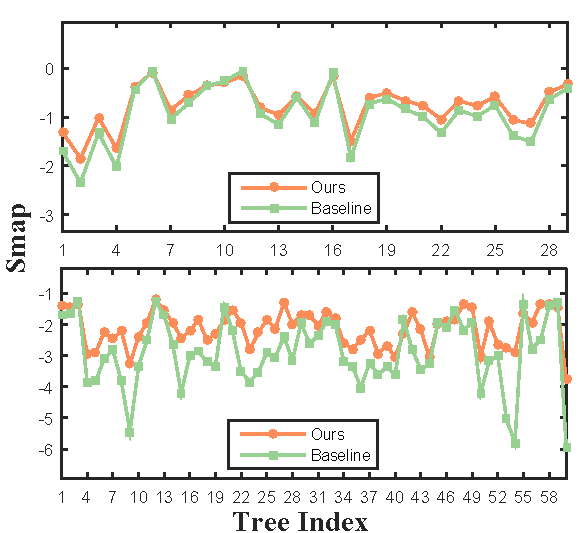
\includegraphics[width=0.7\columnwidth]{fig/v2-Smap-treeindex}
  \vspace{-1mm}
  \caption{
%  \small
  Comparison of tree mapping smoothness.}
  \vspace{-5mm}
  \label{fig:smap}
\end{figure}

\begin{figure*}[b]
	\centering
\vspace{-5mm}
    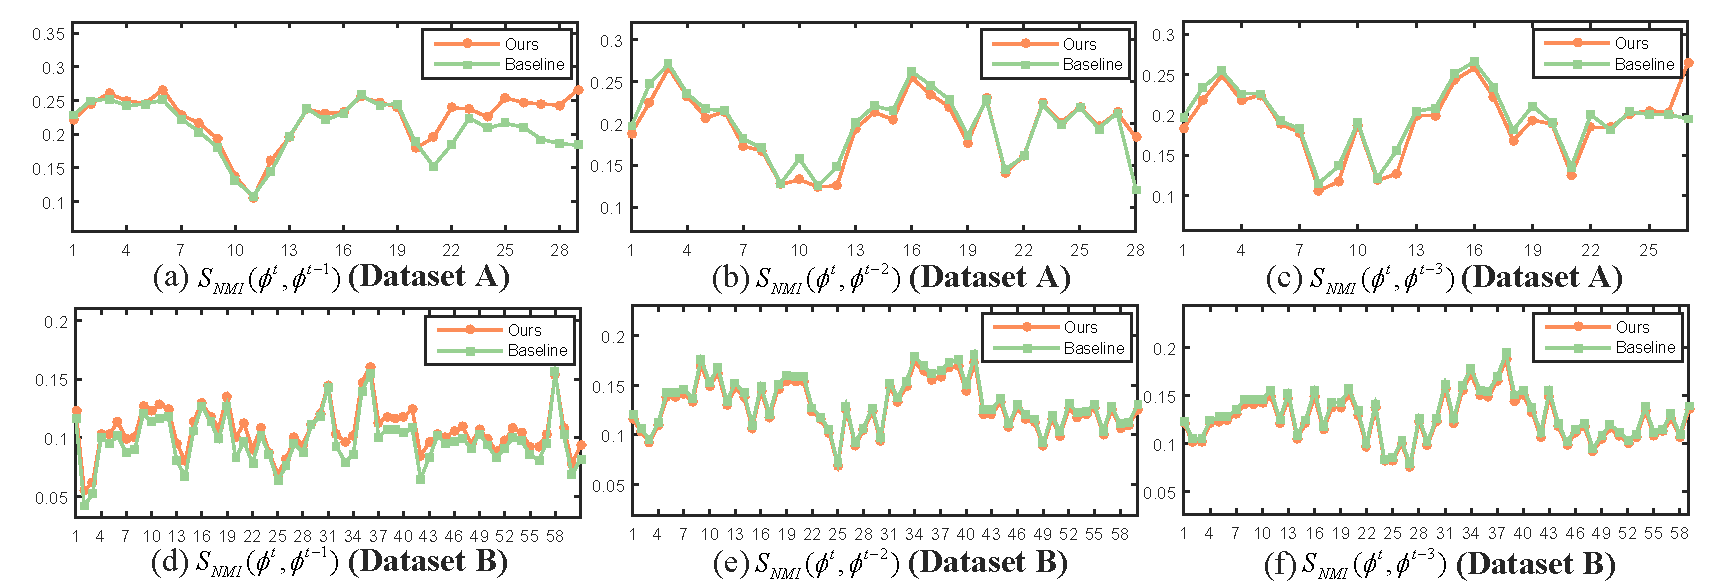
\includegraphics[width=\linewidth]{fig/v2-nmi-treeindex.pdf}
\vspace{-5mm}
	\caption{
%Comparison of NMI smoothness. x-axis represents tree index and y-axis encodes NMI smoothness.
Comparison of NMI smoothness. \kg{X}-axis represents tree index and \kg{Y}-axis encodes NMI smoothness.
}\label{fig:NMI}
\vspace{-3mm}
\end{figure*}

\begin{figure*}[b]
	\centering
    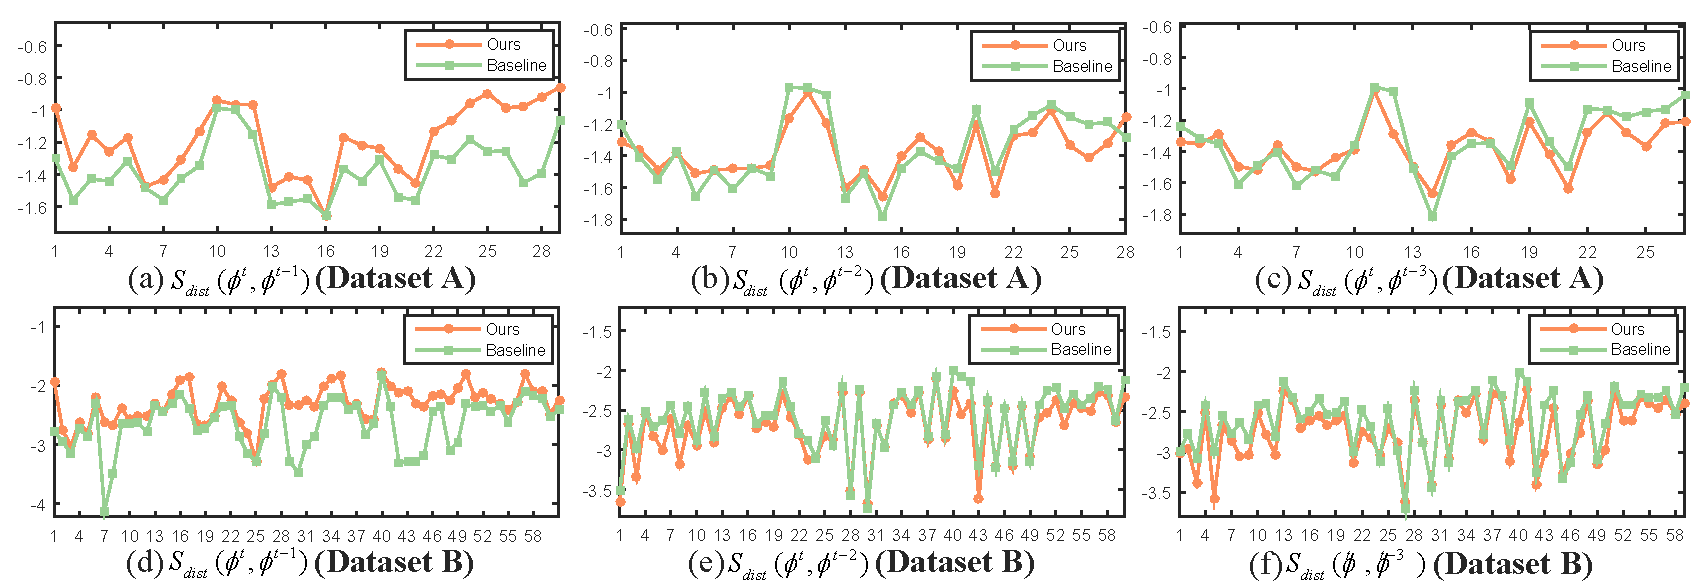
\includegraphics[width=\linewidth]{fig/v2-treedis-treeindex.pdf}
\vspace{-5mm}
	\caption{
%Comparison of tree distance smoothness. y-axis encodes tree distance smoothness.\looseness=-1
Comparison of tree distance smoothness. \kg{Y}-axis encodes tree distance smoothness.\looseness=-1
}\label{fig:distance}
%\vspace{-3mm}
\end{figure*}


%To eliminate the bias caused by the focus node selection, we randomly selected the same number of focus nodes fifty times and ran the experiments fifty times.
To eliminate bias caused by the focus node selection, the same number of focus nodes \kg{was randomly selected 50} times and the experiments \kg{were repeated 50} times.
%At each time, we computed  ${F}$ for each tree cut.
At each time, ${F}$ for each tree cut \kg{was computed}.
%Since the metric ${S_{map}}$ was defined on adjacent tree cuts, we only compute ${S_{map}}$ between adjacent tree cuts.
Since the measure ${S_{map}}$ was defined on adjacent tree cuts, we only \dc{computed} ${S_{map}}$ between adjacent tree cuts.
%\kg{Only} ${S_{map}}$ between adjacent tree cuts \kg{was computed because the metric ${S_{map}}$ was defined on adjacent tree cuts}.
%To demonstrate the global smoothness of our algorithm, ${S_{NMI}}$ and  ${S_{dist}}$ were computed between ${\phi}^t$ and each of ${\phi}^{t-1}$, ${\phi}^{t-2}$, ${\phi}^{t-3}$.
To demonstrate the global smoothness of \kg{the proposed} algorithm, ${S_{NMI}}$ and  ${S_{dist}}$, were computed between ${\phi}^t$ and each of ${\phi}^{t-1}$, ${\phi}^{t-2}$, \kg{and} ${\phi}^{t-3}$.
The results were computed by averaging the 50 trials.



\subsubsection{Results}
\label{sec:results}

%We compared the overall fitness and smoothness with the baseline.
\kg{The} overall fitness and smoothness \kg{were compared} with the baseline.
%As shown in Table~\ref{table:average}, our method can generate a much smoother structure than the baseline while maintaining a larger fitness between ${\phi}^t$ and ${\phi}^{t-1}$.
%As shown in Table~\ref{table:average}, \kg{the proposed} method can generate a much smoother structure than the baseline while maintaining a larger fitness.
As shown in Table~\ref{table:average}, \kg{the proposed} method \docpr{generates} a much smoother structure than the baseline while maintaining \docpr{greater} fitness.
% between ${\phi}^t$ and ${\phi}^{t-1}$.
%When comparing the smoothness between non adjacent tree cuts, our method is a little bit worse.
%When the smoothness between non\kg{-}adjacent tree cuts \kg{were compared}, \kg{the proposed} method \kg{performed slightly} worse\kg{,}
When the smoothness between non\kg{-}adjacent tree cuts \kg{\docpr{was} compared}, \kg{the proposed} method \kg{performed slightly} worse\kg{,}
%This is because our method only considers the adjacent tree cuts to improve the performance for streaming data.
%because \kg{the} method only \kg{considered} the adjacent tree cuts to improve the performance \kg{of data stream}.
because \kg{the} method only \kg{considered} the adjacent tree cuts to improve the performance \dc{of the data stream}.
%focus on streaming data and consider a lot about the treecuts next each other.
%Thus the global smoothness is not maintained to some extent.
Thus\kg{,} the global smoothness \kg{was} not maintained to \kg{a certain} extent.


We further compared the smoothness of our method with the baseline between trees under these measures.
%\kg{The} smoothness of \kg{the} method \kg{was further compared} with the baseline between trees under under these metrics.
%As shown in  Fig.~\ref{fig:smap}, Fig.~\ref{fig:NMI}, and Fig.~\ref{fig:distance}, the proposed streaming algorithm works as well as the baseline under the three metrics for adjacent tree cuts.
%As shown in  Fig.~\ref{fig:smap}, \ref{fig:NMI}, and \ref{fig:distance}, the proposed streaming algorithm works as well as the baseline under the three metrics for adjacent tree cuts.
As shown in  \dc{Figs}.~\ref{fig:smap}, \ref{fig:NMI}, and \ref{fig:distance}, the proposed streaming algorithm worked as well as the baseline under the three measures for adjacent tree cuts.
%For non-adjacent tree cuts, the smoothness of our algorithm is a little bit worse under the metrics ${S_{NMI}}$ and  ${S_{dist}}$.
%commonly used metrics, NMI and tree distance between trees next to each other.
%For non-adjacent tree cuts, the smoothness of \kg{the proposed} algorithm is \kg{slightly} worse under the commonly used metrics NMI and tree distance.
For non-adjacent tree cuts, the smoothness of \kg{the proposed} algorithm \dc{was} \kg{slightly} worse under the commonly used measures NMI and tree distance.
%The fitness of our algorithm at each tree was also evaluated.
The fitness of \kg{the proposed} algorithm at each tree was also evaluated.
%As shown in Fig.~\ref{fig:sf}, our algorithm is much better than the baseline at each time in all the datasets.
%As shown in Fig.~\ref{fig:sf}, \kg{the proposed} algorithm is \kg{more effective} than the baseline at each time in all the datasets.
As shown in Fig.~\ref{fig:sf}, \kg{the proposed} algorithm \dc{was} \kg{more effective} than the baseline at each time in all the datasets.
%This findings demonstrate that our algorithm can preserve the smoothness between adjacent trees as well as the fitness without sacrificing much global smoothness.
%\kg{These} findings demonstrate that \kg{the proposed} algorithm \kg{could} preserve the smoothness between \kg{the} adjacent trees as well as the fitness without sacrificing global smoothness. %\looseness=-1
\kg{These} findings demonstrate that \kg{the proposed} algorithm \docpr{can} preserve the smoothness between \kg{the} adjacent trees as well as the fitness without sacrificing global smoothness. %\looseness=-1

%We compared the overall likelihood and smoothness with the baseline.
%As shown in Table~\ref{table:average}, our method can generate a much smoother structure than the baseline while maintaining a larger likelihood.
%Besides having very good performance under the metric of $\bm{S_{map}}$, our algorithm also achieved a comparable performance under the metrics of $\bm{S_{NMI}}$ and $\bm{S_{dist}}$.
%
%
%Since the metric $\bm{S_{map}}$ is a global smoothness metric, so we further compared our method with the baseline between trees under the metrics $\bm{S_{NMI}}$ and $\bm{S_{dist}}$.
%%First, we assessed the smoothness of our evolutionary tree cut algorithm based on the three different smoothness metrics.
%As shown in Figs.~\ref{fig:NMI} and \ref{fig:distance}, the proposed evolutionary algorithm works pretty well under the commonly used metrics, NMI and tree distance.
%The fitness of our algorithm at each tree was also evaluated.
%As shown in Fig.~\ref{fig:likelihood}, the likelihood of our algorithm is as good as the baseline at each time in all the datasets.
%This findings demonstrate that our algorithm can preserve the smoothness between trees without sacrificing the likelihood of each tree.
%Finally, we demonstrated that the performance of our algorithm consistently improved with the number of focus nodes.
%From Table~\ref{table:average}, we can see that the average likelihood difference decreases with the number of focus nodes, while the average smoothness difference increases with the number of focus nodes.
%This indicates that our algorithm works better when more focus nodes are selected.

\subsection{Scalability}


\begin{figure}[t]
	%\vspace{-2mm}
	\centering
	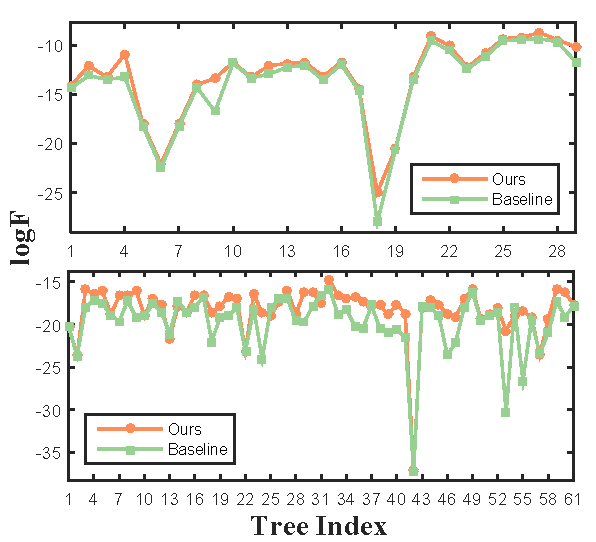
\includegraphics[width=0.7\columnwidth]{fig/v2-Sf-treeindex}
	\vspace{-1mm}
	\caption{
		%  \small
		Comparison of fitness at each tree.}
	\vspace{-6mm}
	\label{fig:sf}
\end{figure}



%In this experiment, we investigate the scalability of our algorithm.
We conducted two experiments to evaluate the scalability of our algorithm.
In the first experiment, we investigated the ability of our algorithm to handle topic trees with a large number of internal nodes ($I_{num}$).
%In the second experiment, we tested the ability of our algorithm to process long sequences of topic trees.
In the \docpr{second, we} tested the ability of our algorithm to process long sequences of topic trees.
%($P_{num}$)

%\tvcgminor{To evaluate the scalability of our algorithm, we investigate how the running time of our algorithm increases with topic tree size and number of topic trees processed.}

%\tvcgminor{\subsubsection{Criteria}}

\subsubsection{Experimental Settings}

%To assess how the running time of our algorithm increases with topic tree size, we generated
%We generated topic trees with different $I_{num}$ by copying the first ten topic trees of Dataset A different times.
%The dataset used in the first experiment was generated by copying the first ten trees in Dataset A by $s$ times ($s\in \{1,3,...,15\}$).
The dataset used in the first experiment was generated by copying the first ten trees in Dataset \docpr{A \emph{\normalsize s}} times ($s\in \{1,3,...,15\}$).
%To generate topic trees with different $I_{num}$, we copied the first ten trees generated using Dataset A by $s$ times ($s\in \{1,3,...,15\}$). %resulting in topic trees with an average $I_{num}$ of $\{118, 354, ..., 1770\}$.
As a result, we obtained eight groups of topic trees with varied $I_{num}$ ($I_{num}\in\{118, 354, ..., 1770\}$). % with the average $I_{num}$ per tree range from 118 to 1770. %of each set range from 118 to 1770. %$\{118, 354, ..., 1770\}$ internal nodes for each tree on average. % internal nodes on average.
For each group of topic trees, we treated the first five trees as old trees and evaluated the average time to process the 6th to 10th trees. %last five topic trees. %the
In our experiments, focus nodes were randomly selected to avoid any biased conditions.
To eliminate randomness caused by the focus node selection, we randomly selected the given number $m$ ($m\in\{1,3,5\}$) of focus nodes 50 times and ran the experiment 50 times.
Results were computed by averaging the 50 trials.

%we randomly selected 50 sets of focus nodes for the same number of focus nodes $m$ ($m\in\{1,3,5\}$).
%The results were calculated by averaging the 50 trials.
%we evaluated the running time under different numbers of focus nodes ($m\in\{1,3,5\}$) and randomly selected 50 sets of focus nodes for each $m$.



In the second experiment, we used the 30 topic trees in Dataset A.
%To assess how the running time of our algorithm increases with $P_{num}$, the 30 topic trees of Dataset A were used.
Specifically, we regarded the first $P_{num}$ ($P_{num}\in \{7,9,...29\}$) trees as old trees, and evaluated the time to process the $(P_{num}+1)$-th tree.
%To eliminate the bias caused by the number of internal nodes in the $(P_{num}+1)$th tree, we normalized the running time by multiplying it with $I_{max}/I_{cur}$
%Other settings are same as the first experiment.
\docpr{All other settings were the} same as the first experiment.
%Similar to the first experiment, we randomly selected 50 sets of focus nodes for each $m\in\{1,3,5\}$ and calculated the results by averaging the 50 trials.\looseness=-1 %repeated the experiments 50 times.



The experiments were run on a workstation with an Intel Xeon E5-2630 CPU (2.4 GHz) and 64GB Memory.


\subsubsection{Results}

As shown in Fig.~\ref{fig:exp-time-Inum}, the running time of our algorithm increases at an approximate quadratic rate with the increase of $I_{num}$.
%our algorithm is able to deal with large topic trees.
%scale well with $I_{num}$.
%For $m=5$, our algorithm can process topic trees with 1770 internal nodes in 66 seconds.
For $m=5$, our algorithm can process topic trees with \docpr{1,770} internal nodes in 66 seconds.
This demonstrates that our algorithm can handle large topic trees.
% shows how the running time increases with $I_{num}$ under different $m$.


%Next, we demonstrate the scalability of our algorithm in regards to $P_{num}$ under different $m$.
Next, we \docpr{demonstrated} the scalability of our algorithm in regards to $P_{num}$ under different \emph{\normalsize m}.
%Here we used normalized running time to eliminate bias caused by different sizes of the topic trees.
\docpr{We} used \docpr{a} normalized running time to eliminate \docpr{any} bias caused by different sizes of the topic trees.
Normalized running time is calculated by multiplying real running time with $(I_{avg}/I_{cur})^2$.
%Here $I_{avg}$ is computing by averaging $I_{num}$ of all trees and $I_{cur}$ is $I_{num}$ of the $(P_{num}+1)$-th topic tree.
Here $I_{avg}$ is \docpr{computed} by averaging $I_{num}$ of all trees and $I_{cur}$ is $I_{num}$ of the $(P_{num}+1)$-th topic tree.
As shown in Fig.~\ref{fig:exp-time-Pnum}, the normalized running time increases slowly with the increase of $P_{num}$ and the results are consistent across different $m$.
This indicates that our algorithm can process long sequences of topic trees efficiently.\looseness=-1

\begin{figure}[t]
%\vspace{-2mm}
\centering
{
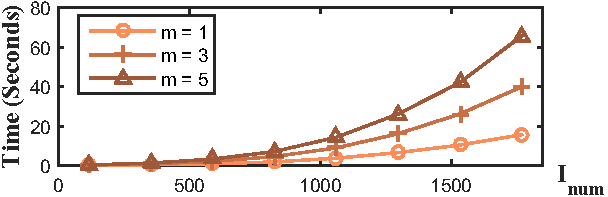
\includegraphics[width=0.36\textwidth]{fig/TotalTime-TopicNumber.pdf}
}
\caption{Running time vs. number of internal nodes in the topic tree ($I_{num}$) vs. number of focus nodes ($m$).}
\label{fig:exp-time-Inum}
\vspace{-1mm}
\end{figure}


\begin{figure}[t]
%\vspace{-2mm}
\centering
{
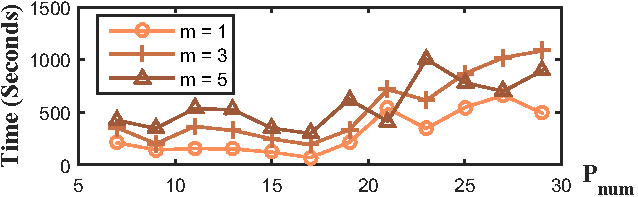
\includegraphics[width=0.36\textwidth]{fig/TotalTime-TreeCount.pdf}
}
\caption{Normalized running time vs. number of topic trees processed ($P_{num}$) vs. number of focus nodes ($m$).}
\label{fig:exp-time-Pnum}
\vspace{-5mm}
\end{figure}

